\section{Auswertung}
\label{sec:Auswertung}

% \begin{figure}
%   \centering
%   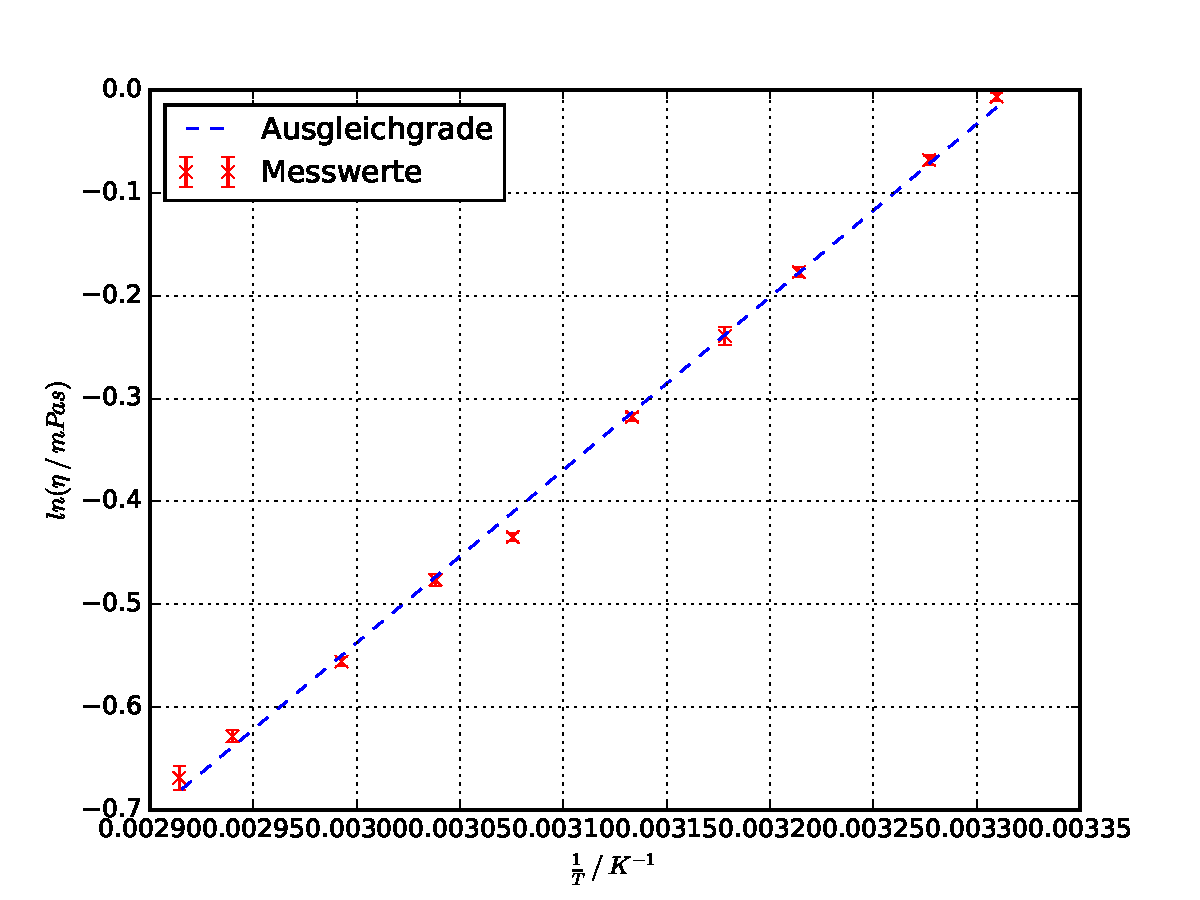
\includegraphics{plot.pdf}
%   \caption{Plot.}
%   \label{fig:plot}
% \end{figure}
\subsection{Charakteristik des Zählrohrs}
Um die Charakteristik des Zählrohrs zu untersuchen wird zu erst die Aktivität
\begin{equation}
 \frac{N_m}{t} = \frac{N}{t} \pm \frac{\sqrt{N}}{t}
 \label{eqn:N}
\end{equation}
bestimmt und mit Fehlerbalcken in ein Diagramm (s. Abb. \ref{fig:char})
eingetragen.Dabei bezeichnet $N_m$ die gemessenen Zerfälle.
Daraus kann dann die Auslösespannung $ U_e = \SI{490}{\volt}$
entnommen werden. Weiter muss nun das \textit{Plateau} \cite{Anleitung}
bestimmt werden, da
dieses den Arbeitsbereich des Zählrohrs kennzeichent. Auf diesem Bereich
des Graphen wird dann eine Ausgleichsgerade
\begin{equation*}
  f\left(x \right) = a \cdot x + b
\end{equation*}
berechnet. Daraus ergibt sich, dass die Steigung $a$ im Plateau
\begin{equation*}
  a = \SI{0.072(7)}{\becquerel\per\volt} \qquad \text{oder} \qquad  a \approx \SI{0.072}{\percent\per\volt}
\end{equation*}
beträgt. Der y-Abschnitt $b$ beträgt dabei
\begin{equation*}
  b = \SI{785(5)}{\becquerel} \;.
\end{equation*}
Alle Werte dazu sind in den Tabellen \ref{tab:a1} und \ref{tab:a2}

\begin{table}
\parbox[t]{0.48\textwidth}{
  \centering
  \caption{Spannungen U und Zählraten N \\ mit Fehler im Überblick(1).}
  \sisetup{round-mode = places , round-precision = 0}
  \begin{tabular}{S[scientific-notation = fixed , fixed-exponent = 0] S[scientific-notation = fixed , fixed-exponent = 0]@{$\pm\qquad$ } S[scientific-notation = fixed , fixed-exponent = 0]}
  \toprule
  $U / \si{\volt}$ & \multicolumn{2}{c}{$N \pm \sqrt{N}$} \\
  \midrule
  % 4.500000000000000000e+02 & 0.000000000000000000e+00 & 0.000000000000000000e+00\\
  % 4.600000000000000000e+02 & 3.000000000000000000e+01 & 5.477225575051661188e+00\\
  % 4.700000000000000000e+02 & 4.713400000000000000e+04 & 2.171036618760724650e+02\\
  4.800000000000000000e+02 & 4.823500000000000000e+04 & 2.196246798517871355e+02\\
  4.900000000000000000e+02 & 4.865700000000000000e+04 & 2.205833175922422242e+02\\
  5.000000000000000000e+02 & 4.879900000000000000e+04 & 2.209049569384987706e+02\\
  5.100000000000000000e+02 & 4.906200000000000000e+04 & 2.214994356651953069e+02\\
  5.200000000000000000e+02 & 4.933800000000000000e+04 & 2.221215883249532226e+02\\
  5.300000000000000000e+02 & 4.932700000000000000e+04 & 2.220968257314813457e+02\\
  5.400000000000000000e+02 & 4.917600000000000000e+04 & 2.217566233509159588e+02\\
  5.500000000000000000e+02 & 4.970400000000000000e+04 & 2.229439391416595697e+02\\
  5.600000000000000000e+02 & 4.993700000000000000e+04 & 2.234658810646493237e+02\\
  5.700000000000000000e+02 & 4.959300000000000000e+04 & 2.226948584947573408e+02\\
  5.800000000000000000e+02 & 5.002100000000000000e+04 & 2.236537502480117041e+02\\
  5.900000000000000000e+02 & 4.974800000000000000e+04 & 2.230425968284982048e+02\\
  6.000000000000000000e+02 & 4.996000000000000000e+04 & 2.235173371351761489e+02\\
  6.100000000000000000e+02 & 4.976400000000000000e+04 & 2.230784615331565419e+02\\
  6.200000000000000000e+02 & 5.010600000000000000e+04 & 2.238436954662784331e+02\\
  6.300000000000000000e+02 & 5.037100000000000000e+04 & 2.244348457793486205e+02\\
  6.400000000000000000e+02 & 5.032700000000000000e+04 & 2.243368003694445179e+02\\
  6.500000000000000000e+02 & 5.021300000000000000e+04 & 2.240825740659009853e+02\\
  \bottomrule
\end{tabular}
\label{tab:a1}
}
\parbox[t]{0.48\textwidth}{
  \caption{Spannungen U und Zählraten N \\ mit Fehler im Überblick (2).}
  \sisetup{round-mode = places , round-precision = 0}
  \begin{tabular}{S[scientific-notation = fixed , fixed-exponent = 0] S[scientific-notation = fixed , fixed-exponent = 0]@{$\pm\qquad$ } S[scientific-notation = fixed , fixed-exponent = 0]}
  \toprule
  $U / \si{\volt}$ & \multicolumn{2}{c}{$N \pm \sqrt{N}$} \\
  \midrule
  6.600000000000000000e+02 & 5.028600000000000000e+04 & 2.242454012906396201e+02\\
  6.700000000000000000e+02 & 5.024600000000000000e+04 & 2.241561955423048289e+02\\
  6.800000000000000000e+02 & 5.010600000000000000e+04 & 2.238436954662784331e+02\\
  6.900000000000000000e+02 & 4.996400000000000000e+04 & 2.235262848078498337e+02\\
  7.000000000000000000e+02 & 4.996600000000000000e+04 & 2.235307585098748859e+02\\
  7.100000000000000000e+02 & 4.978000000000000000e+04 & 2.231143204727119382e+02\\
  7.200000000000000000e+02 & 5.057900000000000000e+04 & 2.248977545463715728e+02\\
  7.300000000000000000e+02 & 5.021800000000000000e+04 & 2.240937303897634649e+02\\
  7.400000000000000000e+02 & 4.985200000000000000e+04 & 2.232756144320288172e+02\\
  7.500000000000000000e+02 & 5.060100000000000000e+04 & 2.249466603441802590e+02\\
  7.600000000000000000e+02 & 5.011100000000000000e+04 & 2.238548636952076549e+02\\
  7.700000000000000000e+02 & 5.055100000000000000e+04 & 2.248354954183168957e+02\\
  7.800000000000000000e+02 & 5.061900000000000000e+04 & 2.249866662715815266e+02\\
  7.900000000000000000e+02 & 5.036200000000000000e+04 & 2.244147945212168906e+02\\
  8.000000000000000000e+02 & 5.055000000000000000e+04 & 2.248332715591711519e+02\\
  8.100000000000000000e+02 & 5.061300000000000000e+04 & 2.249733317528990995e+02\\
  8.200000000000000000e+02 & 5.039100000000000000e+04 & 2.244793977183652487e+02\\
  8.300000000000000000e+02 & 5.063400000000000000e+04 & 2.250199991111901170e+02\\
  8.400000000000000000e+02 & 5.091100000000000000e+04 & 2.256346604580067492e+02\\
  8.500000000000000000e+02 & 5.072300000000000000e+04 & 2.252176724859752142e+02\\
  \bottomrule
\end{tabular}
\label{tab:a2}
}
\end{table}

\begin{figure}
  \centering
  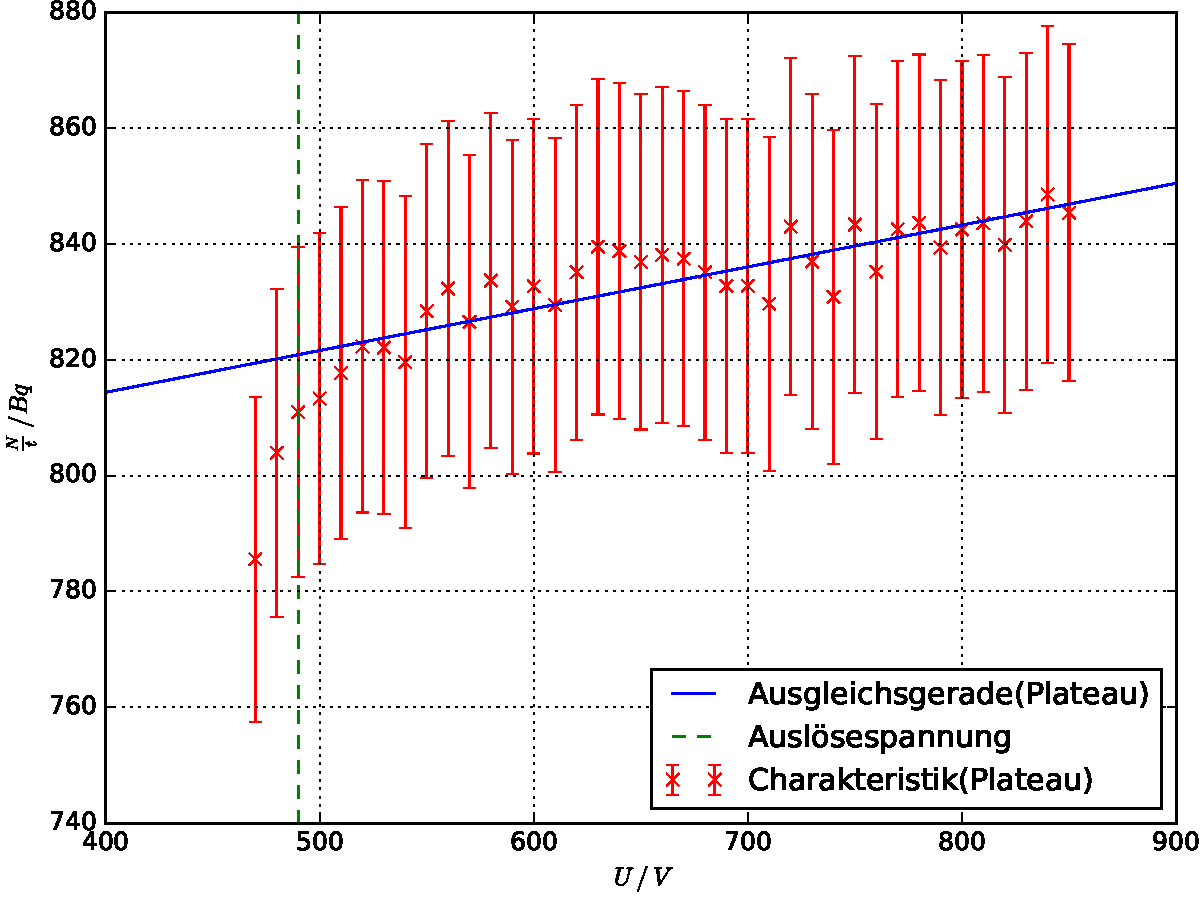
\includegraphics[height= 7cm]{plots/charplot.pdf}
  \caption{Charakteristik des Zählrohr; Zerflälle N gegen die Spannung U aufgetragen.}
  \label{fig:char}
\end{figure}
\subsection{Beobachtung der Nachentladungen und Bestimmung der Totzeit}
Bei der Messung der Totzeit mit einem Oszilloskop ist diese einfach abzulesen.
Die Totzeit $T$ wurde für verschiedene Spannungen bestimmt und gemittelt.
Somit ergibt sich
\begin{equation*}
  T = \SI{232(8)}{\micro\second} \;.
\end{equation*}
Bei der Messung der Totzeit ist auf dem Oszilloskop ein Graph wie in Abbildung
\ref{fig:osz} zu sehen. Der Abfall und somit die Totzeit ist gut zu erkennen.
Die während der Erhohlungszeit auftetenden Impulse können auf die Nachentladungen
zurückgeführt werden.

\begin{figure}
  \centering
  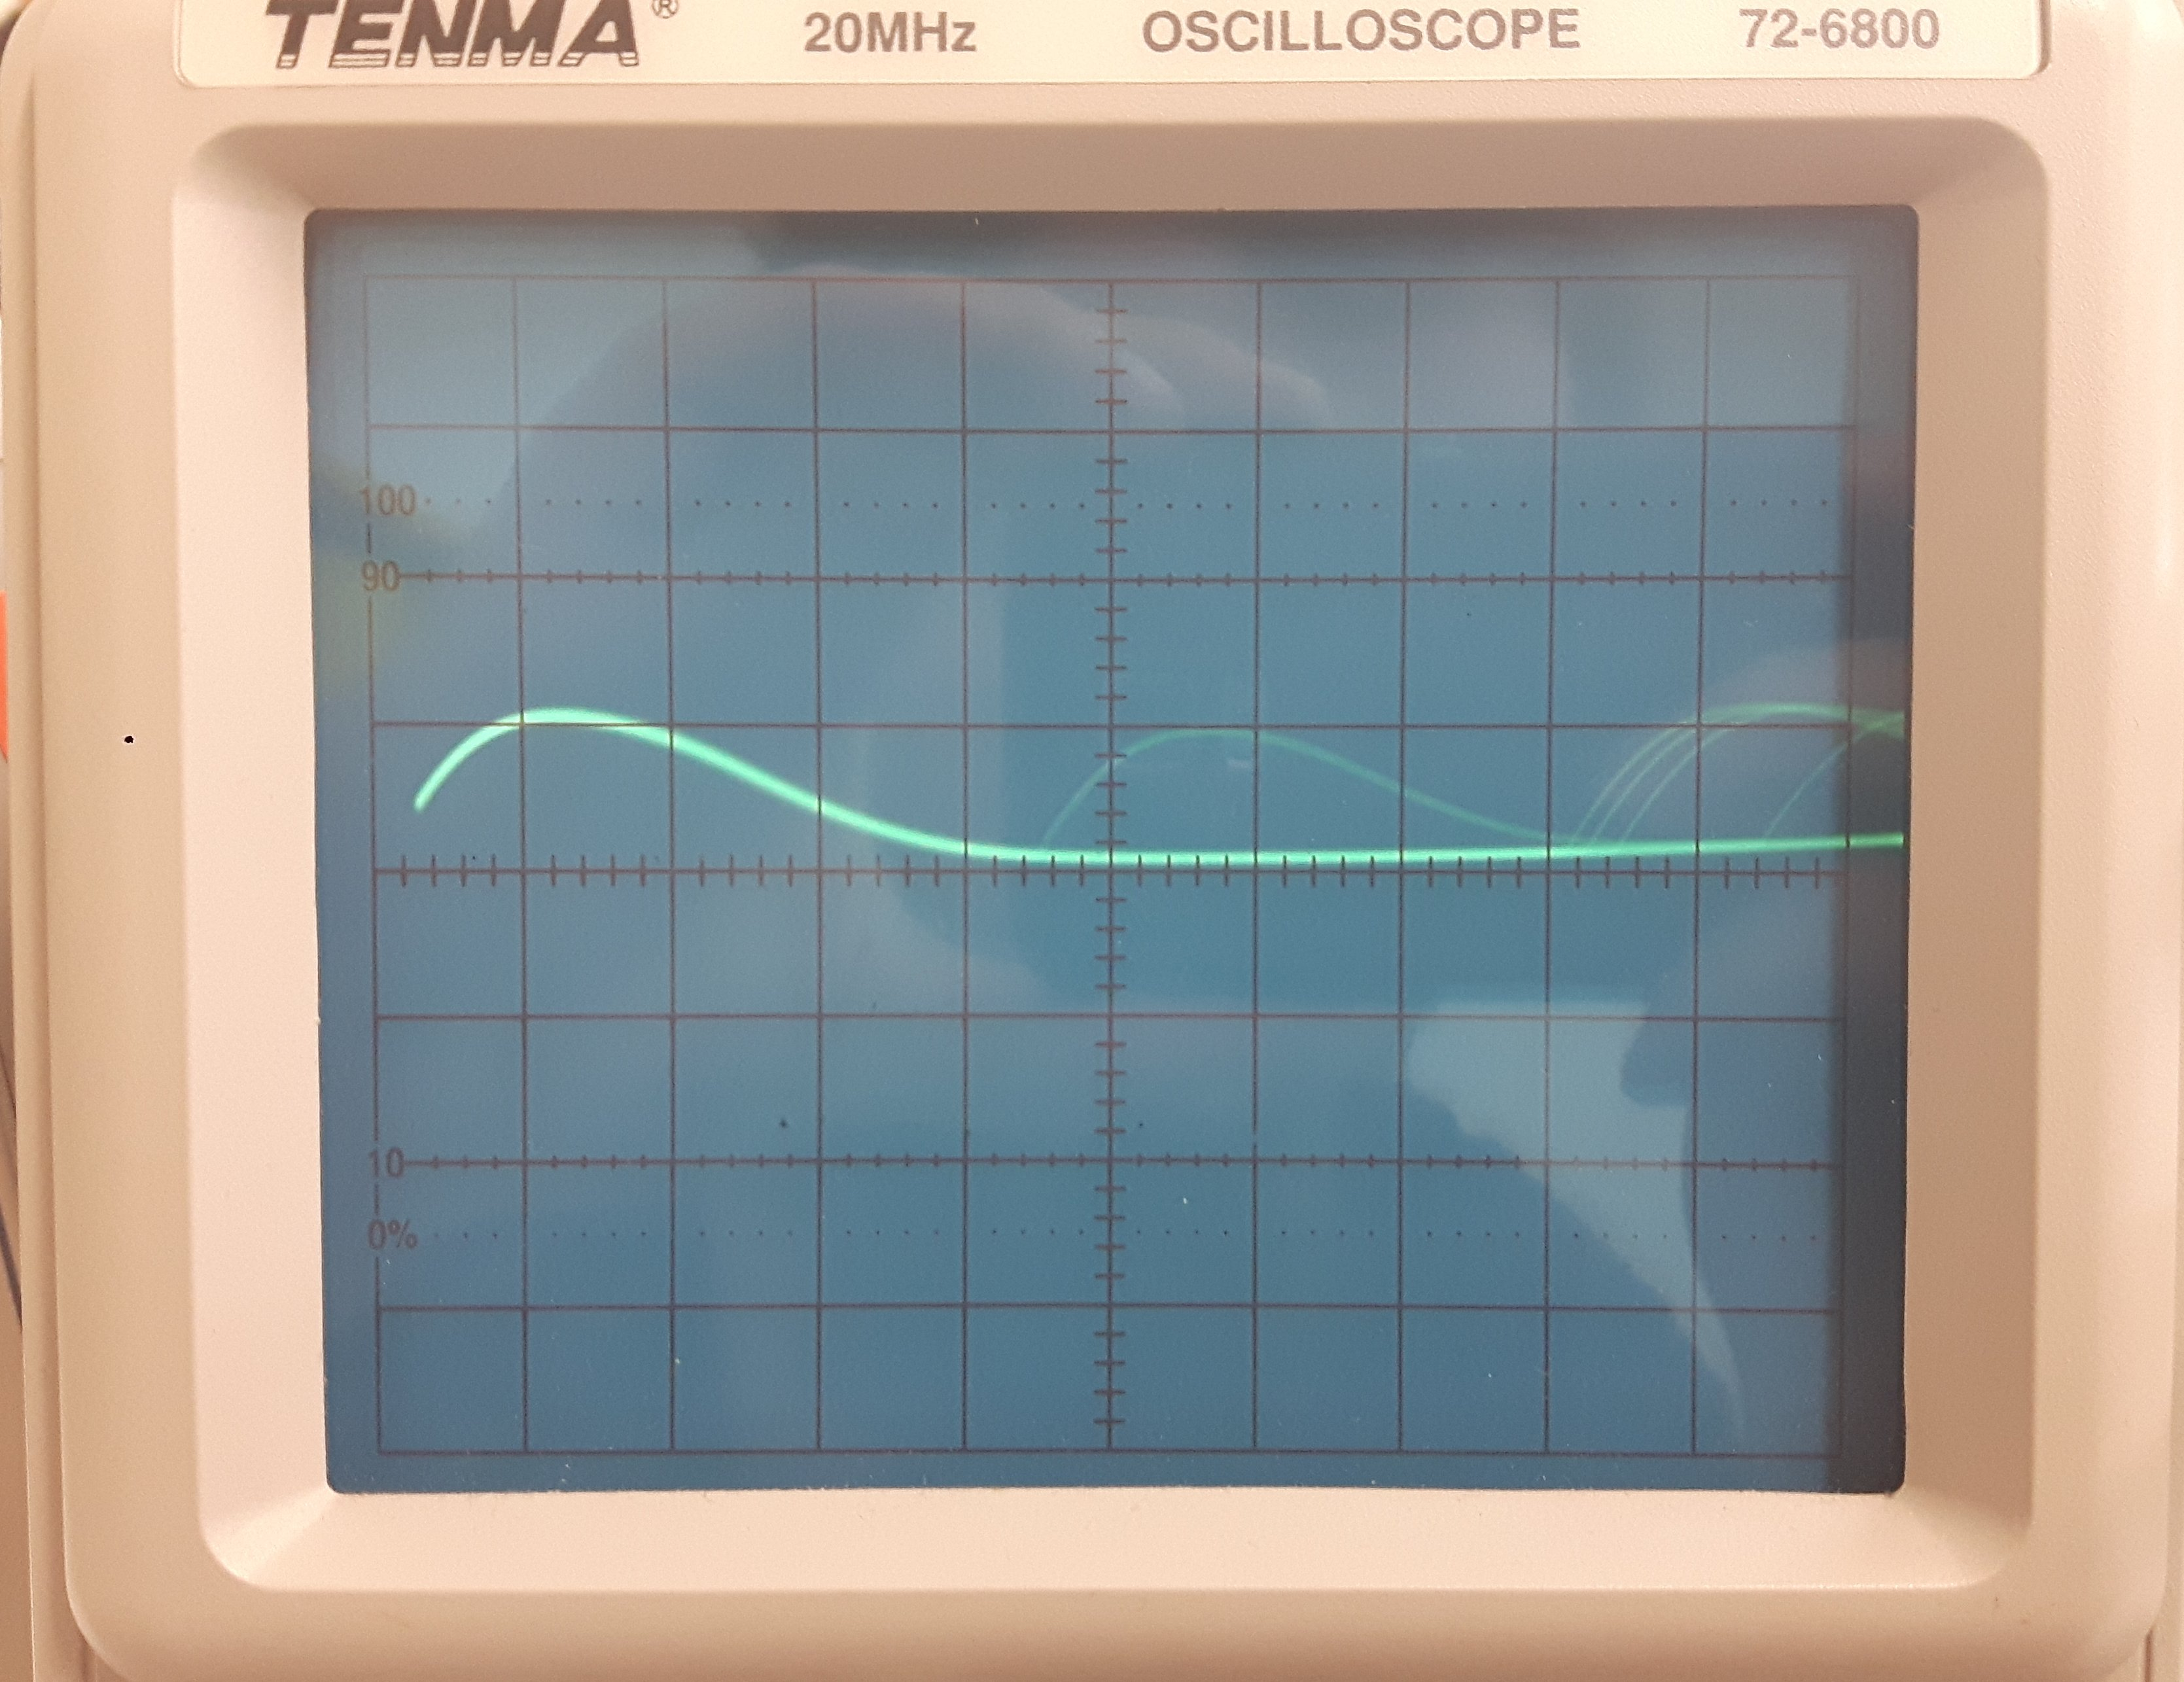
\includegraphics[height = 5cm]{./logos/GM-Oszi.jpg}
  \caption{Bild vom Graphen des Oszilloskop bei der Messung der Totzeit (1 Kästchen horizontal = \texorpdfstring{$\SI{50}{\micro\second}$}{math}).}
  \label{fig:osz}
\end{figure}
\subsection{Bestimmung der Totzeit mit der Zwei-Quellen-Methode}
Aus der Theorie \ref{sec:Theorie} wird die Gleichung \eqref{eqn:easy}
entnommen. Dabei bezeichnet $ N_1 $ die Zählrate des einen Präperats und
$ N_2 $ die des anderen Präperats folglich bezeichnet $N_{1+2}$ die Zählrate
für die Messung bei der beide Präperate gleichzeitig verwendet wurden.
Hier bei beträgt $N_1 = 40048$, $ N_2 = 4039 $ und $N_{1+2} = 43118$.
Werden nun für die Zählraten die selben Fehler angenommen wie in Gleichung
\eqref{eqn:N} dann folgt
\begin{equation*}
  T = \SI{3.0(9)}{\micro\second} \; .
\end{equation*}
\subsection{Bestimmung der freigesetzten Ladungsmenge}
Es gilt der Zusammenhang
\begin{equation*}
  I = \frac{\Delta Q}{\Delta t} \cdot Z \; ,
\end{equation*}
dabei bezeichnet $\Delta Q$ die Ladungsmenge, $\Delta t$ die Messzeit
(hier: $\Delta t = \SI{60}{\second}$) und $Z$ die Anzahl der regrestrierten
Teilchen.
Die Ladungsmenge ergibt sich also mit
\begin{equation*}
  \frac{I \cdot \Delta t}{Z} = \Delta Q \; .
\end{equation*}
Die Ladungsmenge kann auch über die Elementarladung $\symup{e}$ \cite{scipy} ausgedrückt werden mit
\begin{equation*}
M = \frac{\Delta Q}{\symup{e}}\; .
\end{equation*}
Alle Werte und Ergebnisse dazu sind in der Tabelle \ref{tab:e2}
dargestellt.

\begin{table}
  \centering
  \caption{Strom I, Anzahl der Teilchen Z, Ladungsmenge \texorpdfstring{$\Delta Q$}{math} und die Ladungsmenge ausgedrückt über die Elementraladung im Überblick.}
  \sisetup{round-mode = places , round-precision = 2}
  \begin{tabular}{S[scientific-notation=fixed,fixed-exponent = -6 ]@{\qquad} S[scientific-notation=fixed,fixed-exponent = 0, round-precision=0 ] S S[scientific-notation=fixed,fixed-exponent =0 ]}
  \toprule
  $I / \si{\volt}$ & Z & $\Delta Q /\si{\coulomb}$ & $\frac{\Delta Q \cdot10^{10}}{\symup{e}}$ \\
  \midrule
  1.999999999999999909e-07 & 3.000000000000000000e+01 & 4.000000000000000348e-07 & 2.496603650353303294e+02\\
  3.999999999999999819e-07 & 4.713400000000000000e+04 & 5.091865744473204323e-10 & 3.178092651190185247e-01\\
  3.999999999999999819e-07 & 4.823500000000000000e+04 & 4.975640095366435742e-10 & 3.105550306234025060e-01\\
  5.999999999999999728e-07 & 4.865700000000000000e+04 & 7.398729884703126071e-10 & 4.617924009531975127e-01\\
  5.999999999999999728e-07 & 4.879900000000000000e+04 & 7.377200352466239648e-10 & 4.604486332338722510e-01\\
  6.999999999999999683e-07 & 4.906200000000000000e+04 & 8.560596795890912688e-10 & 5.343104302456010979e-01\\
  7.999999999999999638e-07 & 4.933800000000000000e+04 & 9.728809436945154602e-10 & 6.072245288467233992e-01\\
  8.999999999999999593e-07 & 4.932700000000000000e+04 & 1.094735134915968816e-09 & 6.832799335003059138e-01\\
  9.999999999999999547e-07 & 4.917600000000000000e+04 & 1.220107369448511352e-09 & 7.615311280970299412e-01\\
  9.999999999999999547e-07 & 4.970400000000000000e+04 & 1.207146306132303029e-09 & 7.534414686001034145e-01\\
  1.199999999999999946e-06 & 4.993700000000000000e+04 & 1.441816689028175515e-09 & 8.999112022420141521e-01\\
  1.199999999999999946e-06 & 4.959300000000000000e+04 & 1.451817796866493200e-09 & 9.061534028261942764e-01\\
  1.199999999999999946e-06 & 5.002100000000000000e+04 & 1.439395453909358156e-09 & 8.983999861330134173e-01\\
  1.300000000000000047e-06 & 4.974800000000000000e+04 & 1.567902227225215130e-09 & 9.786076059718864517e-01\\
  1.399999999999999937e-06 & 4.996000000000000000e+04 & 1.681345076060848663e-09 & 1.049413063599266671e+00\\
  1.399999999999999937e-06 & 4.976400000000000000e+04 & 1.687967205208584523e-09 & 1.053546271550103830e+00\\
  1.599999999999999928e-06 & 5.010600000000000000e+04 & 1.915938210992695722e-09 & 1.195834582853935180e+00\\
  1.599999999999999928e-06 & 5.037100000000000000e+04 & 1.905858529709555111e-09 & 1.189543340582463582e+00\\
  1.799999999999999919e-06 & 5.032700000000000000e+04 & 2.145965386373119611e-09 & 1.339406254287741627e+00\\
  1.799999999999999919e-06 & 5.021300000000000000e+04 & 2.150837432537390505e-09 & 1.342447146347343967e+00\\
  1.899999999999999808e-06 & 5.028600000000000000e+04 & 2.267032573678558469e-09 & 1.414970449728933266e+00\\
  1.999999999999999909e-06 & 5.024600000000000000e+04 & 2.388249810930222998e-09 & 1.490628298980995137e+00\\
  2.200000000000000112e-06 & 5.010600000000000000e+04 & 2.634415040114956514e-09 & 1.644272551424160955e+00\\
  2.200000000000000112e-06 & 4.996400000000000000e+04 & 2.641902169562084892e-09 & 1.648945650101252935e+00\\
  2.200000000000000112e-06 & 4.996600000000000000e+04 & 2.641796421566665494e-09 & 1.648879647393407755e+00\\
  2.299999999999999578e-06 & 4.978000000000000000e+04 & 2.772197669746885796e-09 & 1.730269705447748940e+00\\
  2.399999999999999891e-06 & 5.057900000000000000e+04 & 2.847031376658296810e-09 & 1.776977231908873467e+00\\
  2.399999999999999891e-06 & 5.021800000000000000e+04 & 2.867497709984467830e-09 & 1.789751312531739913e+00\\
  2.600000000000000094e-06 & 4.985200000000000000e+04 & 3.129262617347348092e-09 & 1.953132118345880297e+00\\
  2.799999999999999873e-06 & 5.060100000000000000e+04 & 3.320092488290744987e-09 & 2.072238756444313879e+00\\
  2.799999999999999873e-06 & 5.011100000000000000e+04 & 3.352557322743509426e-09 & 2.092501712495035804e+00\\
  3.000000000000000076e-06 & 5.055100000000000000e+04 & 3.560760420169729837e-09 & 2.222451865757327560e+00\\
  3.000000000000000076e-06 & 5.061900000000000000e+04 & 3.555977004682036482e-09 & 2.219466292615394298e+00\\
  3.000000000000000076e-06 & 5.036200000000000000e+04 & 3.574123346967952396e-09 & 2.230792348713289019e+00\\
  3.199999999999999855e-06 & 5.055000000000000000e+04 & 3.798219584569733167e-09 & 2.370662219920050440e+00\\
  3.199999999999999855e-06 & 5.061300000000000000e+04 & 3.793491790646671822e-09 & 2.367711363028442317e+00\\
  3.399999999999999634e-06 & 5.039100000000000000e+04 & 4.048341965827230727e-09 & 2.526776332440682893e+00\\
  3.399999999999999634e-06 & 5.063400000000000000e+04 & 4.028913378362364428e-09 & 2.514649961844184656e+00\\
  3.599999999999999837e-06 & 5.091100000000000000e+04 & 4.242698041680579745e-09 & 2.648083854551636751e+00\\
  3.799999999999999616e-06 & 5.072300000000000000e+04 & 4.495002267216055269e-09 & 2.805559767169494290e+00\\
  \bottomrule
\end{tabular}
\label{tab:e2}
\end{table}




















%
